% main.tex — arXiv draft (cs.NE).
%
% Every number in this file is a macro from numbers.tex, which make_tables.py
% writes from prose_numbers.py; every table is \input from tables/, written by
% make_tables.py; every figure is in figures/, written by make_figures.py.
% Nothing quantitative is typed here. Build with ./build.sh.
\documentclass[11pt]{article}

\usepackage[T1]{fontenc}
\usepackage[utf8]{inputenc}
\usepackage{lmodern}
\usepackage[margin=1in]{geometry}
\usepackage{amsmath,amssymb}
\usepackage{graphicx}
\usepackage{booktabs}
\usepackage{array}
\usepackage{xcolor}
\usepackage[round,authoryear]{natbib}
\usepackage{microtype}
\usepackage[hidelinks]{hyperref}
\usepackage{caption}
\captionsetup{font=small,labelfont=bf}

% generated by make_tables.py from prose_numbers.py -- do not edit by hand
% every number in main.tex is one of these macros
\newcommand{\nAsymCapLead}{2/6}  % asym2x: runs in which the first (larger) side wins more than half the cross-population games at the end
\newcommand{\nAsymCapVsSymDelta}{$-$0.33}  % final win rate of the larger side, asym2x vs asym1x: Cliff's delta
\newcommand{\nAsymCapVsSymP}{0.394}  % final win rate of the larger side, asym2x vs asym1x: exact two-sided Mann-Whitney p
\newcommand{\nAsymCross}{0.25}  % share of games crossing populations
\newcommand{\nAsymMutual}{1}  % two-population runs whose BOTH pools end with a member above parity
\newcommand{\nAsymNeither}{7}  % two-population runs where neither pool ends above parity
\newcommand{\nAsymNormLead}{5/6}  % asym2x-norm: runs in which the first (larger) side wins more than half the cross-population games at the end
\newcommand{\nAsymNormVsCapDelta}{$+$0.67}  % final win rate of the larger side, asym2x-norm vs asym2x: Cliff's delta
\newcommand{\nAsymNormVsCapP}{0.065}  % final win rate of the larger side, asym2x-norm vs asym2x: exact two-sided Mann-Whitney p
\newcommand{\nAsymNormVsSymDelta}{$+$0.11}  % final win rate of the larger side, asym2x-norm vs asym1x: Cliff's delta
\newcommand{\nAsymNormVsSymP}{0.818}  % final win rate of the larger side, asym2x-norm vs asym1x: exact two-sided Mann-Whitney p
\newcommand{\nAsymOneSided}{10}  % two-population runs where exactly one pool ends above parity
\newcommand{\nAsymParamLarge}{531}  % parameters of the larger network
\newcommand{\nAsymRunaway}{13}  % two-population runs ending in runaway dominance: cross-population win rate over the last 50,000 games above 0.9 or below 0.1
\newcommand{\nAsymRunawaySym}{4}  % runaways in the symmetric control
\newcommand{\nAsymRuns}{18}  % two-population runs, all conditions
\newcommand{\nAsymSymLead}{4/6}  % asym1x: runs in which the first (larger) side wins more than half the cross-population games at the end
\newcommand{\nAsymWindow}{50,000}  % games over which the final cross-population win rate is averaged
\newcommand{\nBestEndpoint}{$+$0.50}  % highest end-of-run champion (held out) of any single-population run
\newcommand{\nBestEndpointCondition}{es}  % condition of that run
\newcommand{\nBestEndpointLabel}{self-play ES}  % readable name of the condition with the highest endpoint
\newcommand{\nBudget}{500,000}  % self-play games per run
\newcommand{\nCtrlAbovePct}{26}  % control: mean share of checkpoints above parity, in %
\newcommand{\nCtrlBestEndpoint}{$+$0.41}  % highest end-of-run champion (held out) among control seeds
\newcommand{\nCtrlFinalMean}{$-$0.15}  % control: mean end-of-run champion, held out
\newcommand{\nCtrlLagMax}{100,000}  % control: longest internal-to-external lag across seeds
\newcommand{\nCtrlLagMin}{25,000}  % control: shortest internal-to-external lag across seeds
\newcommand{\nCtrlParity}{6/6}  % control: runs with at least one checkpoint above parity
\newcommand{\nCtrlPeakMean}{$+$0.32}  % control: mean best champion, held out
\newcommand{\nCtrlReached}{6/6}  % control: runs whose population ever held 1,500-step rallies
\newcommand{\nCtrlRuns}{6}  % number of control seeds
\newcommand{\nCtrlTInternalMax}{415,000}  % control: latest internal transition across seeds
\newcommand{\nCtrlTInternalMedian}{120,000}  % control: median internal transition
\newcommand{\nCtrlTInternalMin}{55,000}  % control: earliest internal transition across seeds
\newcommand{\nCtrlTInternalRatio}{7.5}  % control: latest / earliest internal transition
\newcommand{\nCtrlTParityMax}{440,000}  % control: latest first-above-parity checkpoint across seeds
\newcommand{\nCtrlTParityMin}{85,000}  % control: earliest first-above-parity checkpoint across seeds
\newcommand{\nCyclicCtrlPct}{0.2}  % control: cyclic share of decided checkpoint triads, pooled, in %
\newcommand{\nCyclicLearningMaxPct}{0.2}  % largest pooled cyclic share among conditions in which every run learned to rally, in %
\newcommand{\nEsAbovePct}{7}  % es: mean share of checkpoints above parity, in %
\newcommand{\nEsCandidates}{50}  % self-play ES: mirrored perturbations per iteration
\newcommand{\nEsFinalMean}{$-$2.08}  % es: mean end-of-run champion, held out
\newcommand{\nEsParity}{2/6}  % es: runs with at least one checkpoint above parity
\newcommand{\nEsPeakMean}{$-$1.56}  % es: mean best champion, held out
\newcommand{\nEsReached}{4/6}  % es: runs whose population ever held 1,500-step rallies
\newcommand{\nEsSdRatio}{3.5}  % es: s.d. across seeds of the end-of-run champion (held out), relative to the control's
\newcommand{\nFamilySdRatioMax}{3.5}  % largest endpoint s.d. ratio (vs control) among the other three families
\newcommand{\nFamilySdRatioMin}{3.0}  % smallest endpoint s.d. ratio (vs control) among the other three families
\newcommand{\nGaAbovePct}{3}  % ga2015: mean share of checkpoints above parity, in %
\newcommand{\nGaElitePct}{20}  % generational GA: share retained per generation, in %
\newcommand{\nGaFinalMean}{$-$2.00}  % ga2015: mean end-of-run champion, held out
\newcommand{\nGaOpponents}{10}  % generational GA: games per individual per generation
\newcommand{\nGaParity}{5/6}  % ga2015: runs with at least one checkpoint above parity
\newcommand{\nGaPeakMean}{$-$0.68}  % ga2015: mean best champion, held out
\newcommand{\nGaPop}{100}  % generational GA: population
\newcommand{\nGaReached}{5/6}  % ga2015: runs whose population ever held 1,500-step rallies
\newcommand{\nGaSdRatio}{3.0}  % ga2015: s.d. across seeds of the end-of-run champion (held out), relative to the control's
\newcommand{\nHaPublished}{$+$0.35}  % Ha (2020): published score of the same GA at the same budget (literature constant)
\newcommand{\nHidden}{10}  % hidden units per layer, standard network
\newcommand{\nHiddenLarge}{16}  % hidden units per layer, larger network
\newcommand{\nHofCapFull}{512}  % archive capacity spanning the whole run
\newcommand{\nHofEvery}{1,000}  % games between archive entries
\newcommand{\nHofP}{0.25}  % probability of an archive game, main archive conditions
\newcommand{\nHofWindow}{50,000}  % games over which early and late archive win rates are averaged
\newcommand{\nHofparentAbovePct}{2}  % hof-0.25: mean share of checkpoints above parity, in %
\newcommand{\nHofparentFinalMean}{$-$4.10}  % hof-0.25: mean end-of-run champion, held out
\newcommand{\nHofparentOtherReached}{0/4}  % archive as parent at p = 0.5 or with a full-run archive: runs that learned to rally, pooled
\newcommand{\nHofparentParity}{1/6}  % hof-0.25: runs with at least one checkpoint above parity
\newcommand{\nHofparentPeakMean}{$-$3.94}  % hof-0.25: mean best champion, held out
\newcommand{\nHofparentReached}{1/6}  % hof-0.25: runs whose population ever held 1,500-step rallies
\newcommand{\nHofparentRegressPct}{12.0}  % archive as parent: share of all games that copy an archived genome back into the pool (p x archive win rate), in %
\newcommand{\nHoftestAbovePct}{18}  % hof-eval-v2: mean share of checkpoints above parity, in %
\newcommand{\nHoftestFinalMean}{$-$1.01}  % hof-eval-v2: mean end-of-run champion, held out
\newcommand{\nHoftestNFailed}{1}  % archive as test: runs that never learned to rally
\newcommand{\nHoftestParity}{4/6}  % hof-eval-v2: runs with at least one checkpoint above parity
\newcommand{\nHoftestPeakMean}{$-$0.55}  % hof-eval-v2: mean best champion, held out
\newcommand{\nHoftestReached}{5/6}  % hof-eval-v2: runs whose population ever held 1,500-step rallies
\newcommand{\nHoftestSdRatio}{3.1}  % hof-eval-v2: s.d. across seeds of the end-of-run champion (held out), relative to the control's
\newcommand{\nHoftestSkipLateLearnedMax}{22}  % archive as test, runs that learned: highest late share of games without a selection event, in %
\newcommand{\nHoftestSkipLateLearnedMin}{21}  % archive as test, runs that learned: lowest late share of games without a selection event, in %
\newcommand{\nHoftestSkipLateMax}{22}  % archive as test: highest per-seed share of games without a selection event, last 50,000 games, in %
\newcommand{\nHoftestSkipLateMin}{12}  % archive as test: lowest per-seed share of games without a selection event, last 50,000 games, in %
\newcommand{\nHoftestTInternalMedian}{150,000}  % archive as test: median internal transition of the runs that learned
\newcommand{\nHoftestVsCtrlAboveDelta}{$-$0.33}  % archive as test vs control, above_parity: Cliff's delta
\newcommand{\nHoftestVsCtrlAboveP}{0.370}  % archive as test vs control, above_parity: exact two-sided Mann-Whitney p
\newcommand{\nHoftestVsCtrlFinalDelta}{$-$0.28}  % archive as test vs control, final_holdout: Cliff's delta
\newcommand{\nHoftestVsCtrlFinalP}{0.485}  % archive as test vs control, final_holdout: exact two-sided Mann-Whitney p
\newcommand{\nHoftestVsCtrlLateDelta}{$-$0.22}  % archive as test vs control, late_mean: Cliff's delta
\newcommand{\nHoftestVsCtrlLateP}{0.589}  % archive as test vs control, late_mean: exact two-sided Mann-Whitney p
\newcommand{\nHoftestVsCtrlPeakDelta}{$+$0.00}  % archive as test vs control, peak_holdout: Cliff's delta
\newcommand{\nHoftestVsCtrlPeakP}{1.000}  % archive as test vs control, peak_holdout: exact two-sided Mann-Whitney p
\newcommand{\nHoftestWinEarlyMax}{0.50}  % archive as test: highest per-seed archive win rate, first 50,000 games
\newcommand{\nHoftestWinEarlyMin}{0.46}  % archive as test: lowest per-seed archive win rate, first 50,000 games
\newcommand{\nHoftestWinLateFailed}{0.50}  % archive as test, runs that never learned: mean late archive win rate
\newcommand{\nHoftestWinLateLearnedMax}{0.16}  % archive as test, runs that learned: highest late archive win rate
\newcommand{\nHoftestWinLateLearnedMin}{0.11}  % archive as test, runs that learned: lowest late archive win rate
\newcommand{\nHoftestWinLateMax}{0.50}  % archive as test: highest per-seed archive win rate, last 50,000 games
\newcommand{\nHoftestWinLateMin}{0.11}  % archive as test: lowest per-seed archive win rate, last 50,000 games
\newcommand{\nInitScale}{0.5}  % s.d. of the initial weights
\newcommand{\nLateWindow}{100,000}  % games in the late window of every metric
\newcommand{\nLives}{5}  % lives per side
\newcommand{\nLongRally}{1,500}  % self-play rally length that counts as learned
\newcommand{\nMinPSix}{0.002}  % smallest attainable two-sided exact p with six runs a side
\newcommand{\nNAct}{3}  % buttons (network outputs)
\newcommand{\nNCkpt}{100}  % checkpoints per run
\newcommand{\nNRunsTotal}{59}  % independent runs analysed (a two-population run counts once)
\newcommand{\nNSingleRuns}{41}  % single-population runs analysed
\newcommand{\nObsSize}{12}  % observation size
\newcommand{\nParamCount}{273}  % parameters of the evolved policy
\newcommand{\nPop}{128}  % population size of the control
\newcommand{\nPopBig}{512}  % population sweep: larger population (defined, never run)
\newcommand{\nPopEvery}{50,000}  % games between population snapshots
\newcommand{\nPopSmall}{32}  % population sweep: smaller population
\newcommand{\nPopSmallRuns}{1}  % runs of the smaller population
\newcommand{\nProxyEndAbove}{67}  % final snapshot: mean number of pool members above parity
\newcommand{\nProxyEndExported}{$-$0.08}  % final snapshot: mean score of the exported individual
\newcommand{\nProxyGap}{0.90}  % mean gap, best individual in the pool minus exported, points per episode
\newcommand{\nProxyPop}{128}  % population size in the proxy check
\newcommand{\nProxyRankMean}{60}  % mean rank of the exported individual in its own pool (1 = best), all snapshots
\newcommand{\nProxyRho}{$+$0.06}  % mean Spearman rho(streak counter, score vs baseline) over snapshots
\newcommand{\nProxyRuns}{6}  % control runs with population snapshots
\newcommand{\nReexportBestLevel}{$-$1.14}  % mean score of the best member (oracle) over all snapshots
\newcommand{\nReexportBudgetPct}{0.8}  % largest ranking budget as a share of one run's games, in %
\newcommand{\nReexportGamesMax}{4,096}  % ranking games per snapshot at the largest internal round robin
\newcommand{\nReexportMedianLevel}{$-$1.83}  % mean score of the population's median member over all snapshots
\newcommand{\nReexportPeersMax}{64}  % largest internal round robin: peers per individual
\newcommand{\nReexportRecMax}{65}  % share of the exported-to-best gap closed by the largest internal round robin, in %
\newcommand{\nReexportRhoMax}{$+$0.57}  % rho(internal margin, true skill) at the largest round robin
\newcommand{\nReexportRhoStreak}{$+$0.04}  % rho(streak counter, true skill) in the re-export analysis
\newcommand{\nReexportStreakLevel}{$-$1.95}  % mean score of the streak-exported individual over all snapshots
\newcommand{\nRefFinalHoldout}{$+$0.04}  % reference run: final checkpoint, re-scored on the held-out seed
\newcommand{\nRefLag}{67,800}  % reference run: games between the two transitions
\newcommand{\nRefPeakHoldout}{$+$0.50}  % reference run: best checkpoint, re-scored on the held-out seed
\newcommand{\nRefTInternal}{104,200}  % reference run: first game count at which self-play rallies exceed 1,500 steps
\newcommand{\nRefTParity}{172,000}  % reference run: first checkpoint scoring above 0 against the 2015 baseline
\newcommand{\nRhoWithinCtrl}{$+$0.74}  % control: mean over seeds of Spearman rho(within-run Elo, training time)
\newcommand{\nRunawayCut}{0.9}  % win rate beyond which a two-population run is a runaway (and its complement)
\newcommand{\nRunawayPct}{90}  % runaway cut as a percentage of games
\newcommand{\nRunsMax}{6}  % most runs of any analysed condition
\newcommand{\nRunsMin}{1}  % fewest runs of any analysed condition
\newcommand{\nSaveEvery}{5,000}  % games between exported checkpoints
\newcommand{\nSeedsMain}{6}  % seeds of the conditions that carry a claim
\newcommand{\nSelectEpisodes}{1,000}  % episodes per held-out re-score
\newcommand{\nSigbigAbovePct}{11}  % sigma-0.20: mean share of checkpoints above parity, in %
\newcommand{\nSigbigReached}{2/3}  % sigma-0.20: runs that learned to rally
\newcommand{\nSigbigVolReachedDelta}{$-$0.17}  % sigma-0.20 vs control, volatility over runs that learned: Cliff's delta
\newcommand{\nSigbigVolReachedP}{0.857}  % sigma-0.20 vs control, volatility over runs that learned: exact p
\newcommand{\nSigma}{0.1}  % mutation scale of the control
\newcommand{\nSigmaBig}{0.20}  % mutation-scale sweep: larger sigma
\newcommand{\nSigmaCtrl}{0.10}  % control sigma, two decimals
\newcommand{\nSigmaSmall}{0.05}  % mutation-scale sweep: smaller sigma
\newcommand{\nSigsmallAbovePct}{26}  % sigma-0.05: mean share of checkpoints above parity, in %
\newcommand{\nSigsmallReached}{3/3}  % sigma-0.05: runs that learned to rally
\newcommand{\nSigsmallVolReachedDelta}{$+$0.00}  % sigma-0.05 vs control, volatility over runs that learned: Cliff's delta
\newcommand{\nSigsmallVolReachedP}{1.000}  % sigma-0.05 vs control, volatility over runs that learned: exact p
\newcommand{\nSweepEpisodes}{200}  % episodes per checkpoint in the sweep
\newcommand{\nTLimit}{3,000}  % episode step limit
\newcommand{\nValGames}{200}  % paired games in the bit-level check
\newcommand{\nValRefCoreHours}{13}  % core-hours for one 500,000-game run at the reference implementation's measured games per second
\newcommand{\nValSpeedup}{26}  % compiled / reference games per second on one core
\newcommand{\nValSteps}{304,812}  % environment steps compared


% marks text that waits on data; must be empty before submission
\newcommand{\PENDING}[1]{\textcolor{red}{[PENDING: #1]}}
\newcommand{\cond}[1]{\texttt{#1}}

\title{What a self-playing population learns, what it forgets,\\
       and which of the two you measure}
\author{Roland Loechli}
\date{Draft, \today}

\begin{document}
\maketitle

\begin{abstract}
In a self-play genetic algorithm, the individual exported as ``the champion''
is close to a median member of its own population, and much of what looks like
coevolutionary instability in its learning curve is noise added by the rule
that picks it. We show this for David Ha's tournament-selection algorithm on
Slime Volleyball, run as a designed experiment rather than a single run:
\nNRunsTotal{} independent runs of \nBudget{} self-play games, in a compiled
environment that reproduces the reference implementation bit for bit, with
every agent scored against a frozen opponent never seen in training. Ha's export
rule promotes the individual with the longest winning lineage; scored against
its whole population, that individual ranks on average \nProxyRankMean{} of
\nProxyPop, its lineage counter is uncorrelated with its skill
($\rho=\nProxyRho$), and the best member of the same pool is \nProxyGap{}
points per episode better. The population itself is not cycling: skill is
almost perfectly transitive across checkpoints. Internal improvement precedes
any external transfer by tens of thousands of games, and the timing of the
phase change varies \nCtrlTInternalRatio-fold across seeds. An archive of past
champions used as a parent abolishes learning; used as a test, it
\PENDING{C5b from hof-eval-v2}. Algorithm families differ in reliability, not
ceiling. A two-population variant with unequal capacity is reported as
exploratory. Any evolutionary loop that promotes one artefact out of a
population, including LLM-driven program evolution, has the same exposure; we
state this as a hypothesis and give the diagnostic.
\end{abstract}

% =========================================================================
\section{Introduction}

Self-play evolution produces competent agents from an entirely internal signal.
In the steady-state genetic algorithm that \citet{ha2020slimevolleygym} uses
for Slime Volleyball, two members of a population of \nPop{} play one game, the
loser is overwritten by a mutated copy of the winner, and that is all: nothing
in the loop refers to an absolute standard of play. Run for \nBudget{} games, it
produces an agent that holds the expert policy shipped with the environment to
a draw. The learning curve by which this is usually reported, the score of an
exported champion against that expert, is also strikingly unstable: competence
is reached, lost and regained between adjacent checkpoints.

The textbook explanation is coevolutionary forgetting. Fitness is relative, so
a skill that no current opponent punishes is not selected for and can be lost,
and the population cycles \citep{cliff1995tracking,popovici2012coevolutionary};
the standard remedy is a hall of fame of past champions to test against
\citep{rosin1997new}. This paper asks where the instability actually lives, and
answers with a design rather than a run: \nNRunsTotal{} runs across conditions
that each change one thing, a pre-registered evaluation protocol, and
measurements the external learning curve cannot make.

The main finding is that the explanation is wrong here and the instability is
mostly a reporting artefact. Ha's algorithm exports the individual with the
longest winning lineage, by design ``without actually computing who is best to
save time'' \citep{ha2020slimevolleygym}. Because the lineage counter is
inherited by the loser on every replacement, it measures the age of a lineage,
not the merit of an individual. Scored against the whole population, the
exported champion is a middling member of it, and the population contains
individuals almost a point per episode better. Meanwhile a round robin of every
checkpoint against every other shows skill to be almost perfectly transitive:
later champions beat earlier ones, and the population is not going in circles.
In \citeauthor{miconi2009why}'s \citeyearpar{miconi2009why} terms, historical
progress is steady; what fluctuates is our estimate of global progress, and
it fluctuates because of which individual we chose to measure.

\paragraph{Contributions.}
\begin{enumerate}
\item The export rule, not coevolution, is the dominant noise source in the
  reported curve (\S\ref{sec:export}); an internal round robin recovers most of
  the loss cheaply.
\item Internal improvement precedes external transfer by tens of thousands of
  games, and the phase change is robust in occurrence but not in timing
  (\S\ref{sec:lag}, \S\ref{sec:timing}).
\item An archive used as a parent abolishes learning; used as a test it
  \PENDING{C5b} (\S\ref{sec:archive}).
\item Four algorithm families reach a similar ceiling and differ in how
  reliably they reach it (\S\ref{sec:families}).
\item An exploratory two-population block with unequal capacity
  (\S\ref{sec:asym}).
\item A compiled port of the environment, validated bit for bit, and an
  analysis pipeline in which every number is generated and checked against the
  raw files (\S\ref{sec:repro}).
\end{enumerate}

\paragraph{Related work.}
Measuring progress in coevolution is an old problem: \citet{cliff1995tracking}
introduced tests of current individuals against ancestral opponents,
\citet{miconi2009why} separated local, historical and global progress, and
recent work compares archive-based methods for global progress
\citep{simione2020longterm,nolfi2025global} and examines how a hall of fame can
make progress look larger than it is \citep{seals2026tripping}. Memory
mechanisms range from the hall of fame \citep{rosin1997new} to Pareto and
Nash-based archives \citep{ficici2001pareto,ficici2003memory}; disengagement
between unequal populations is studied by \citet{cartlidge2004combating}. In
symmetric zero-sum games, any game decomposes into a transitive and a cyclic
part \citep{balduzzi2019openended}, and real games appear to be transitive at
the extremes of skill with cycles concentrated in between
\citep{czarnecki2020spinning}. On the evaluation side, single-seed results in
reinforcement learning have repeatedly been shown to mislead
\citep{henderson2018matters,agarwal2021precipice}. What we add is a measurement
of the step that all of these take as given: which individual is reported.

% =========================================================================
\section{Setup}
\label{sec:setup}

\paragraph{Task.}
Slime Volleyball is a two-player, zero-sum, symmetric game
\citep{ha2015slime}, used here through \texttt{slimevolleygym}
\citep{ha2020slimevolleygym}. Each agent observes an \nObsSize-dimensional state in its
own frame and presses \nNAct{} binary buttons. An episode ends when a side loses
\nLives{} lives or after \nTLimit{} steps; its score is points won minus points
lost, in $[-\nLives,\nLives]$. Every evolved agent is the same fixed
\nObsSize--\nHidden--\nHidden--\nNAct{} $\tanh$ network with \nParamCount{}
parameters. Nothing but the weights evolves.

\paragraph{External yardstick.}
The environment ships a small recurrent policy evolved by \citet{ha2015slime}.
It is never used in training. Every checkpoint is scored against it over
\nSweepEpisodes{} episodes on one evaluation seed; the final and the best
checkpoint of each run are re-scored over \nSelectEpisodes{} episodes on a
disjoint seed, because the best of \nNCkpt{} checkpoints is a selected
maximum. All headline numbers are held out. The
protocol was fixed before the runs and is recorded with the data.

\paragraph{The control algorithm.}
A faithful replication of Ha's tournament-selection GA: population \nPop,
initial weights $\mathcal N(0,\nInitScale^2)$, mutation $\sigma=\nSigma$.
Each of \nBudget{} games
draws two members; the loser is replaced by a mutant of the winner and
inherits the winner's streak counter, which then grows by one; a tie mutates
one player in place. Every \nSaveEvery{} games the member with the largest streak is
exported, giving \nNCkpt{} checkpoints per run.

\paragraph{Conditions.}
Each condition changes one thing (Table~\ref{tab:conditions}). Seed counts
differ by design: \nSeedsMain{} for every condition that carries a claim, fewer for side
conditions that were cut when the design was revised. Every change after the
first run started is recorded, with what was known at the time, in a decision
log that ships with the data.

\begin{table}[t]
\centering\small
\caption{Conditions analysed. Two-population runs count once per seed.}
\label{tab:conditions}
% generated by make_tables.py from the markdown table -- do not edit
\begin{tabular}{l>{\raggedright\arraybackslash}p{0.66\linewidth}r}
\toprule
condition & what it changes relative to the control & runs \\
\midrule
\texttt{control} & Ha's 2020 GA: population 128, $\sigma$ = 0.1, champion = longest winning streak & 6 \\
\texttt{hof-eval-v2} & archive as test: with p = 0.25 the opponent is an archived champion (capacity 512); genes come only from the living pool & 6 \\
\texttt{hof-0.25} & archive as parent: with p = 0.25 the opponent is an archived champion (capacity 64) whose mutant replaces a member it beats & 6 \\
\texttt{hof-0.50} & archive as parent: with p = 0.5 the opponent is an archived champion (capacity 64) whose mutant replaces a member it beats & 1 \\
\texttt{hof-full} & archive as parent: with p = 0.25 the opponent is an archived champion (capacity 512) whose mutant replaces a member it beats & 3 \\
\texttt{ga2015} & generational GA: population 100, 10 games per individual per generation, top 20 kept, uniform crossover, $\sigma$ = 0.1 & 6 \\
\texttt{es} & self-play OpenAI-ES: 50 mirrored perturbations, 4 games each, learning rate 0.03, $\sigma$ = 0.1; reports the mean & 6 \\
\texttt{sigma-0.05} & mutation scale $\sigma$ = 0.05 & 3 \\
\texttt{sigma-0.20} & mutation scale $\sigma$ = 0.2 & 3 \\
\texttt{pop-32} & population 32 & 1 \\
\texttt{asym1x} & two populations of 128, 273 v 273 parameters, $\sigma$ = 0.100 v 0.100; a share 0.25 of games crosses populations & 6 \\
\texttt{asym2x} & two populations of 128, 531 v 273 parameters, $\sigma$ = 0.100 v 0.100; a share 0.25 of games crosses populations & 6 \\
\texttt{asym2x-norm} & two populations of 128, 531 v 273 parameters, $\sigma$ = 0.072 v 0.100; a share 0.25 of games crosses populations & 6 \\
\bottomrule
\end{tabular}

\end{table}

\paragraph{Measurements.}
Beyond the learning curve, three measurements need no external opponent:
(i)~a round robin of a run's checkpoints, spaced \nPopEvery{} games apart, with
Bradley--Terry ratings \citep{bradley1952rank} on the Elo scale and a count of
cyclic triads; (ii)~for the control, which snapshots its whole population every
\nPopEvery{} games, every member is scored against the yardstick and compared with
the exported one; (iii)~the internal transition, the first point at which the
population's own training games last more than \nLongRally{} steps. Comparisons use
the exact two-sided Mann--Whitney test with full enumeration
\citep{mann1947test} and Cliff's $\delta$ as effect size; with \nSeedsMain{} runs a
side the smallest attainable $p$ is \nMinPSix. Secondary comparisons are uncorrected for
multiplicity. Because a run that never learns has no volatility, every
stability comparison is also reported over the runs that learned.

% =========================================================================
\section{Results}
\label{sec:results}

\begin{table}[t]
\centering\small
\caption{Headline results. Points per episode against the 2015 policy, mean
$\pm$ s.e.m.\ across runs, held out. ``Learned to rally'': the population ever
held \nLongRally-step rallies against itself. The last two rows are the single run
on the unmodified environment and Ha's published value.}
\label{tab:headline}
\resizebox{\linewidth}{!}{% generated by make_tables.py from the markdown table -- do not edit
\begin{tabular}{>{\raggedright\arraybackslash}p{0.24\linewidth}r>{\raggedleft\arraybackslash}p{0.13\linewidth}>{\raggedleft\arraybackslash}p{0.13\linewidth}>{\raggedleft\arraybackslash}p{0.13\linewidth}>{\raggedleft\arraybackslash}p{0.13\linewidth}}
\toprule
condition & runs & learned to rally & best champion (held out) & end-of-run champion & checkpoints above parity \\
\midrule
control (Ha 2020 GA) & 6 & 6/6 & +0.32 $\pm$ 0.06 & $-$0.15 $\pm$ 0.27 & 26\% \\
archive as test, full span & 6 & 5/6 & $-$0.55 $\pm$ 0.86 & $-$1.01 $\pm$ 0.83 & 18\% \\
archive as parent, p=0.25 & 6 & 1/6 & $-$3.94 $\pm$ 0.90 & $-$4.10 $\pm$ 0.74 & 2\% \\
archive as parent, p=0.50 & 1 & 0/1 & $-$4.84 $\pm$ --- & $-$4.84 $\pm$ --- & 0\% \\
archive as parent, full span & 3 & 0/3 & $-$4.83 $\pm$ 0.01 & $-$4.84 $\pm$ 0.00 & 0\% \\
generational GA (Ha 2015) & 6 & 5/6 & $-$0.68 $\pm$ 0.83 & $-$2.00 $\pm$ 0.82 & 3\% \\
self-play ES & 6 & 4/6 & $-$1.56 $\pm$ 0.99 & $-$2.08 $\pm$ 0.94 & 7\% \\
sigma = 0.05 & 3 & 3/3 & +0.34 $\pm$ 0.07 & $-$0.17 $\pm$ 0.23 & 26\% \\
sigma = 0.20 & 3 & 2/3 & $-$1.44 $\pm$ 1.70 & $-$1.66 $\pm$ 1.60 & 11\% \\
population 32 & 1 & 0/1 & $-$4.84 $\pm$ --- & $-$4.86 $\pm$ --- & 0\% \\
\emph{reference run, unmodified environment} & 1 & 1/1 & \emph{+0.50 $\pm$ 0.03} & \emph{+0.04 $\pm$ 0.02} & \emph{22\%} \\
\emph{Ha (2020), same algorithm and budget} & 1 & --- & \emph{+0.35 $\pm$ 0.02} & --- & --- \\
\bottomrule
\end{tabular}
}
\end{table}

\subsection{Internal improvement precedes external transfer}
\label{sec:lag}

The reference run, Ha's algorithm at Ha's budget on the unmodified environment,
has two regimes (Figure~\ref{fig:reference}). At first its champion loses
almost every point to the 2015 policy; then it climbs steeply and starts
producing champions that beat it. The internal signal moves first: the
population's own rallies pass \nLongRally{} steps at
\nRefTInternal{} games, and the first champion above parity appears at
\nRefTParity, a lag of \nRefLag{} games. An evaluation stopped in between
reports total failure from a population that is already improving. Held out,
the best checkpoint scores \nRefPeakHoldout{} and the final one
\nRefFinalHoldout, against Ha's published \nHaPublished{} for the same
algorithm and budget.

\begin{figure}[t]
\centering
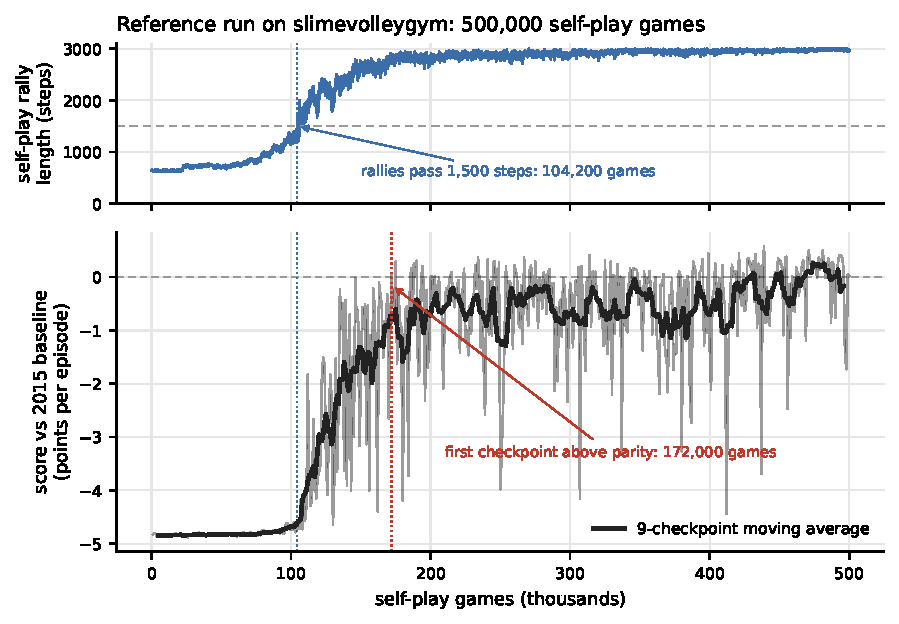
\includegraphics[width=0.85\linewidth]{figures/fig1_reference_trajectory.pdf}
\caption{The reference run. Top: rally length of the population's training
games against itself. Bottom: score of the exported champion against the 2015
policy, every checkpoint (thin) and a moving average (thick). Dotted lines mark
the internal transition and the first checkpoint above parity.}
\label{fig:reference}
\end{figure}

\subsection{The phase change is robust; its timing is not}
\label{sec:timing}

Across \nCtrlRuns{} control seeds the internal transition happens anywhere from
\nCtrlTInternalMin{} to \nCtrlTInternalMax{} games, a
\nCtrlTInternalRatio-fold spread, and the first above-parity checkpoint from
\nCtrlTParityMin{} to \nCtrlTParityMax{} (Figure~\ref{fig:seeds}). The lag
between them is always present, \nCtrlLagMin{} to \nCtrlLagMax{} games. Every
seed reaches the same band (\nCtrlReached{} learned to rally, \nCtrlParity{}
produced an above-parity champion), so the occurrence of the transition
replicates and its timing does not. A single run supports no claim about when
self-play starts working, although the first version of this study, with
one seed, reported a single transition time.

\begin{figure}[t]
\centering
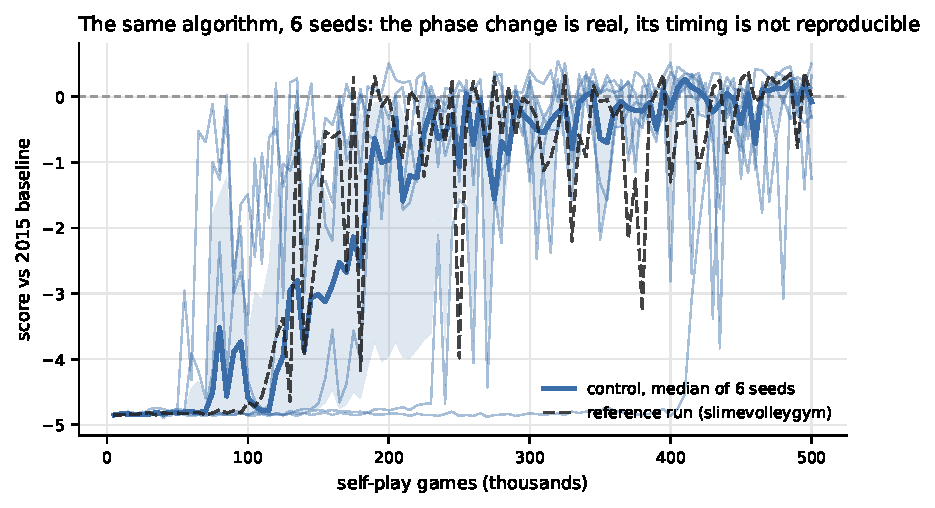
\includegraphics[width=0.85\linewidth]{figures/fig2_control_seeds.pdf}
\caption{Every control seed (thin), median and inter-quartile band (thick), and
the reference run on the same checkpoint grid (dashed).}
\label{fig:seeds}
\end{figure}

\subsection{The population is not cycling}
\label{sec:transitive}

If the swings were forgetting, later champions should not reliably beat
earlier ones, and the checkpoint tournament should contain cycles. Neither is
the case (Figure~\ref{fig:transitive}). Within control runs the rank
correlation between Elo and training time averages \nRhoWithinCtrl, and
\nCyclicCtrlPct\% of decided checkpoint triads are cyclic; no condition whose
runs all learned exceeds \nCyclicLearningMaxPct\%. Only the archive-as-parent
runs, which never learned, show substantial intransitivity: their champions are
equally bad policies whose pairwise results are noise. The game, at the scale
of skill explored here, is dominated by its transitive component
\citep{balduzzi2019openended,czarnecki2020spinning}.

\begin{figure}[t]
\centering
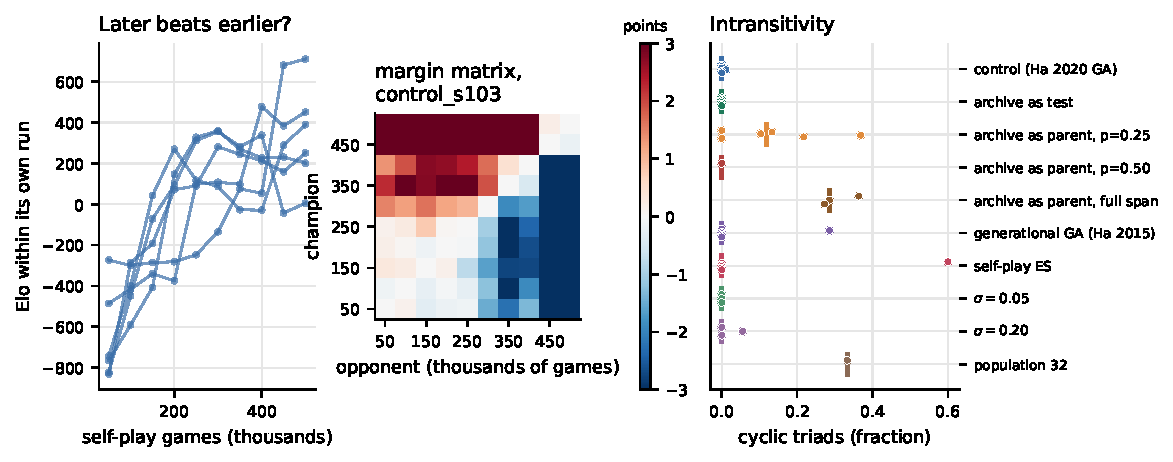
\includegraphics[width=\linewidth]{figures/fig5_coevolution.pdf}
\caption{Left: Elo of each checkpoint within its own run, control seeds. Middle:
pairwise margin matrix of one control run, later checkpoints against earlier.
Right: share of decided checkpoint triads that are cyclic, per condition.}
\label{fig:transitive}
\end{figure}

\subsection{The export rule is the noise source}
\label{sec:export}

Because the control snapshots its whole population, the exported champion can
be compared with every individual it was chosen from
(Figure~\ref{fig:export}). Over \nProxyRuns{} seeds and all snapshots, the
exported individual ranks on average \nProxyRankMean{} of \nProxyPop{} in its
own pool. The rank correlation between the streak counter and actual skill is
\nProxyRho, and the best member of the same pool is \nProxyGap{} points per
episode better. At the last snapshot the exported champion averages
\nProxyEndExported{} while \nProxyEndAbove{} of its peers are above parity. The
counter cannot do better: it is inherited on every replacement, so it records
how long a lineage has survived, not how good its current member is. In a
separate re-scoring of the same snapshots, the streak rule (\nReexportStreakLevel)
does no better than picking the population's median member
(\nReexportMedianLevel); the best member averages \nReexportBestLevel.

The rule can be replaced without external information. Ranking the pool by an
internal round robin of \nReexportGamesMax{} games per snapshot,
\nReexportBudgetPct\% of the training budget, closes \nReexportRecMax\% of the gap between the exported
and the best member (Appendix, Table~\ref{tab:reexport}). Its correlation with
true skill saturates near \nReexportRhoMax: internal fitness measures skill
against the current population, which is not the same as skill against an
unseen opponent, so held-out evaluation remains necessary for selection as
well as for reporting.

\begin{figure}[t]
\centering
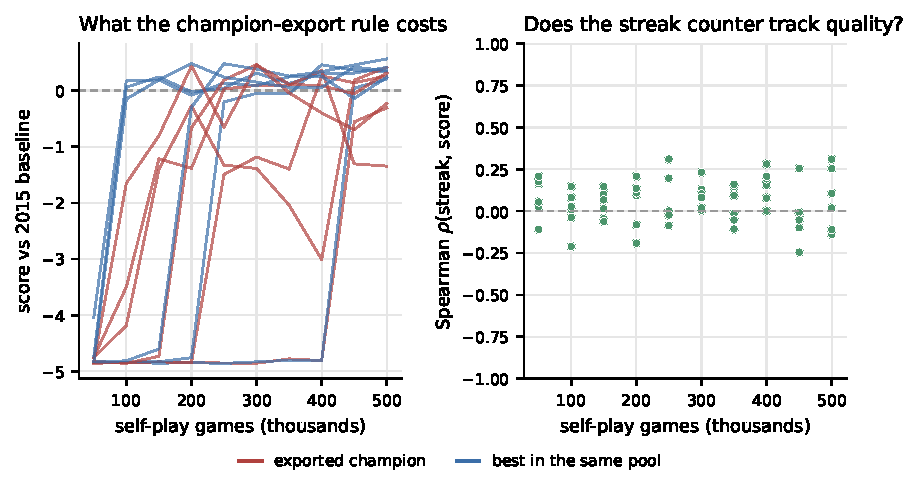
\includegraphics[width=0.9\linewidth]{figures/fig6_champion_proxy.pdf}
\caption{Left: the exported champion (red) and the best member of the same
population (blue), every control seed. Right: Spearman correlation between the
streak counter and score against the 2015 policy, every seed and snapshot.}
\label{fig:export}
\end{figure}

\subsection{An archive of past champions: as a parent, and as a test}
\label{sec:archive}

The standard remedy for forgetting is a hall of fame \citep{rosin1997new}. We
tested two readings of it. Our first implementation applied Ha's replacement
rule to archive games, so a winning archived genome became the parent of the
member it beat: an archive used as a \emph{parent}. With $p=\nHofP$ that copies
an old genotype back into the pool in \nHofparentRegressPct\% of all games, and
it abolishes learning: \nHofparentReached{} runs learned to rally, against
\nCtrlReached{} for the control, and \nHofparentOtherReached{} at a higher dose
or with a full-run archive (Table~\ref{tab:headline}). These runs are also the
most ``stable'' in the matrix, with near-zero volatility and drawdown, which is
why stability is only compared among runs that learned.

The literature's reading uses the archive as a \emph{test}: archived champions
are opponents, never parents. In \cond{hof-eval-v2} an archive game that the
population member loses costs it its slot, but the replacement comes from the
living pool; the archive holds a champion from every \nHofEvery{} games of the
run (capacity \nHofCapFull).
\PENDING{C5b paragraph from hof-eval-v2: reached \nHoftestReached, parity
\nHoftestParity, peak \nHoftestPeakMean, final \nHoftestFinalMean, above
\nHoftestAbovePct\%, archive win rate early \nHoftestWinEarlyMin--\nHoftestWinEarlyMax{}
late \nHoftestWinLateMin--\nHoftestWinLateMax, games without selection late
\nHoftestSkipLateMin--\nHoftestSkipLateMax\%, vs control above $p=\nHoftestVsCtrlAboveP$,
$\delta=\nHoftestVsCtrlAboveDelta$.}
An earlier version of this condition carried a streak-accounting bug that
changed which champions entered the archive; its runs are superseded and
excluded, and the change in the claim is recorded in the decision log.

\begin{figure}[t]
\centering
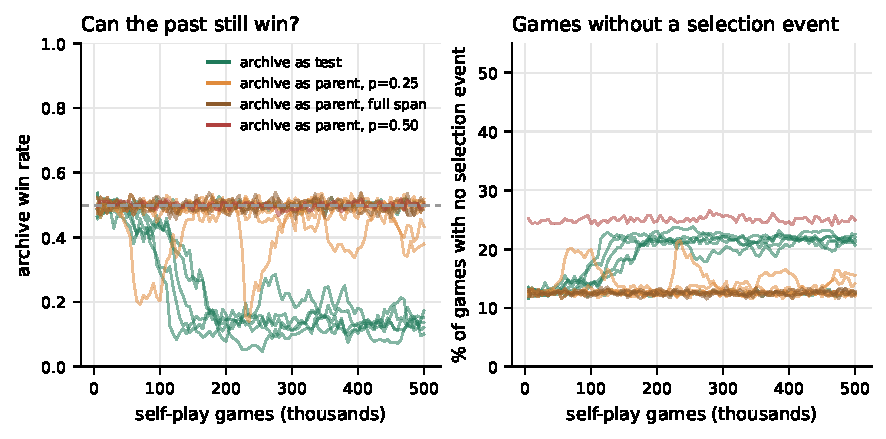
\includegraphics[width=0.9\linewidth]{figures/fig10_archive_decay.pdf}
\caption{Left: the archive's win rate against the current population, every
archive run. Right: the share of games that produce no selection event,
because an archive game the population member wins overwrites nothing.}
\label{fig:archive}
\end{figure}

\subsection{Algorithm families differ in reliability, not ceiling}
\label{sec:families}

Two further families change the machinery with policy and environment fixed: a
generational GA in the style of Ha's 2015 experiment, which ranks by an
explicitly computed fitness and uses crossover, and a self-play evolution
strategy \citep{salimans2017evolution,ha2017estool}, which reports its
distribution mean and so has no export rule at all (Figure~\ref{fig:families}).
\PENDING{C6 recheck with hof-eval-v2 as the fourth family: reached
\nCtrlReached{} / \nGaReached{} / \nEsReached{} / \nHoftestReached; parity
\nCtrlParity{} / \nGaParity{} / \nEsParity{} / \nHoftestParity; s.d.\ ratio of
endpoints \nGaSdRatio, \nEsSdRatio, \nHoftestSdRatio; best endpoint
\nBestEndpoint{} (\nBestEndpointCondition) vs best control \nCtrlBestEndpoint.}
The self-play ES was tuned only at pilot scale, so its result is a statement
about the configuration we could afford, not about the method.

\begin{figure}[t]
\centering
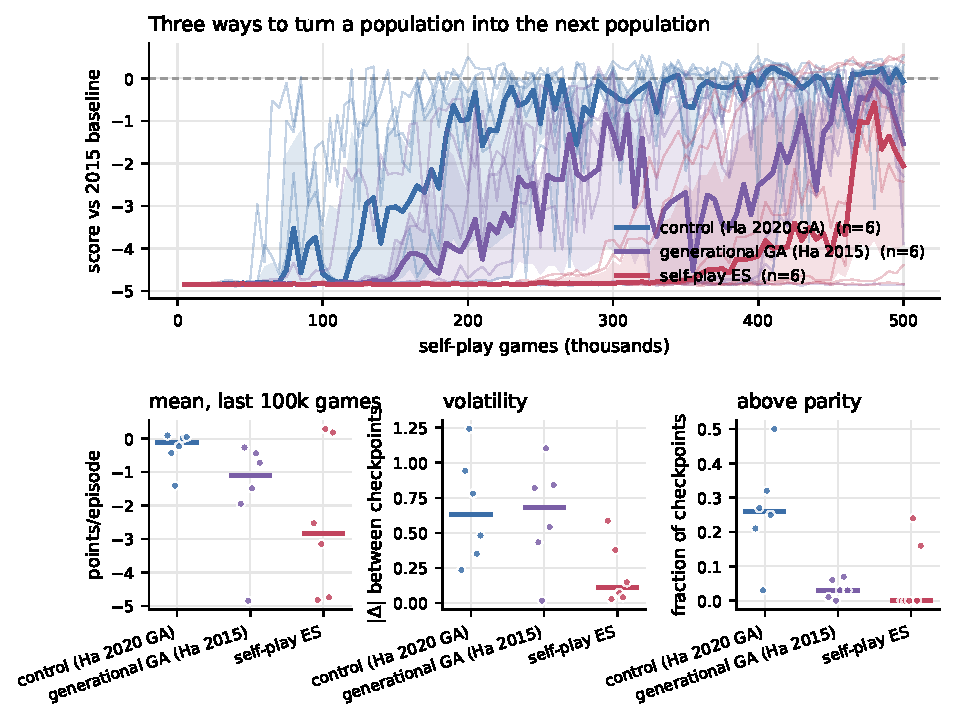
\includegraphics[width=0.9\linewidth]{figures/fig8_algorithm_families.pdf}
\caption{Three families at an identical budget. Top: median and inter-quartile
band. Bottom: per-seed level and volatility of the last \nLateWindow{} games and the
share of checkpoints above parity.}
\label{fig:families}
\end{figure}

% =========================================================================
\section{Unequal power (exploratory)}
\label{sec:asym}

This block was designed after the main matrix had run and re-implemented twice
before the runs reported here; it is exploratory and we draw no confirmatory
conclusion from it. Two populations of \nPop{} play only each other, a share
\nAsymCross{} of each side's games crossing over; in two conditions one side
has a \nObsSize--\nHiddenLarge--\nHiddenLarge--\nNAct{} network with
\nAsymParamLarge{} parameters against \nParamCount, in one with a common per-parameter
$\sigma$ and in one with the larger side's $\sigma$ scaled to equalise the
mutation step norm. A symmetric two-population control has \nParamCount{} a side
(Figure~\ref{fig:asym}, Table~\ref{tab:asym}).

Of \nAsymRuns{} runs, \nAsymMutual{} ended with both pools holding a member
above parity; \nAsymOneSided{} ended with exactly one, \nAsymNeither{} with
neither. \nAsymRunaway{} ended in runaway dominance (one side winning more
than a share \nRunawayCut{} of the cross-population games at the end), \nAsymRunawaySym{} of them in the symmetric
control, where the sides differ only in their seed. Neither capacity condition
is distinguishable from that control (common $\sigma$: $\delta=\nAsymCapVsSymDelta$,
$p=\nAsymCapVsSymP$; matched step: $\delta=\nAsymNormVsSymDelta$,
$p=\nAsymNormVsSymP$). The larger side led in \nAsymCapLead{} runs at common
$\sigma$ and in \nAsymNormLead{} with the step norm matched ($\delta=\nAsymNormVsCapDelta$,
$p=\nAsymNormVsCapP$), which suggests, but at \nSeedsMain{} seeds a side does not
establish, that extra capacity converts into advantage only when the mutation
scale is adjusted to it. The pattern of one side collapsing is consistent with
disengagement \citep{cartlidge2004combating}.

\begin{figure}[t]
\centering
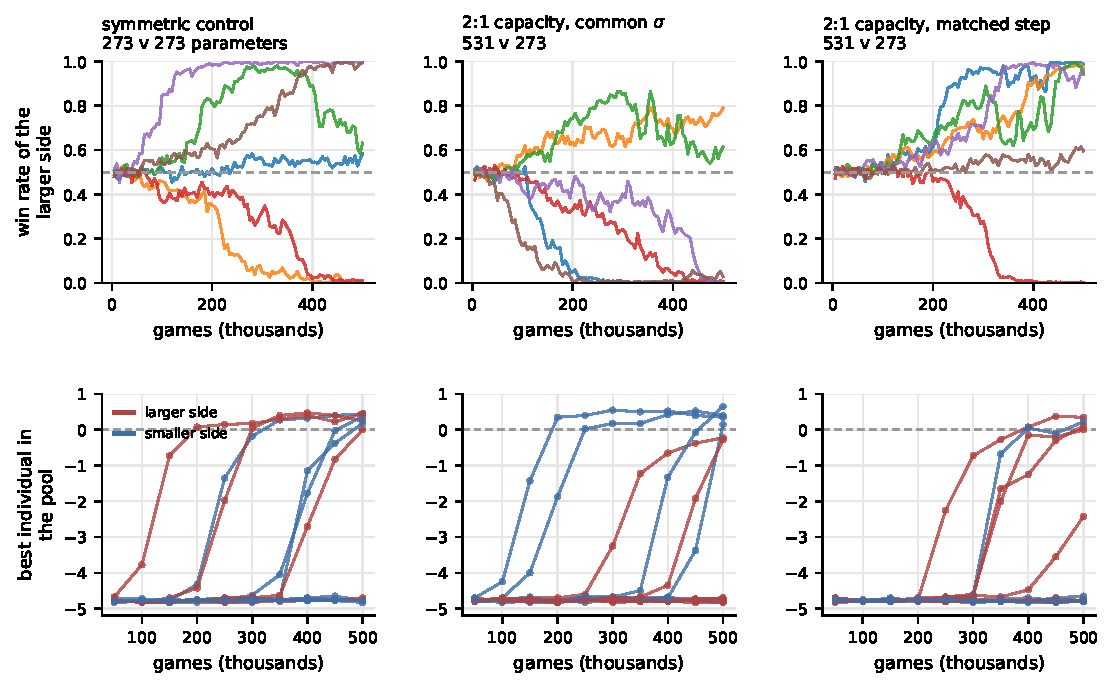
\includegraphics[width=0.9\linewidth]{figures/fig11_asymmetric.pdf}
\caption{Two-population runs. Top: the larger side's win rate in
cross-population games, one line per seed. Bottom: the best member of each pool
against the 2015 policy (red: larger side, blue: smaller).}
\label{fig:asym}
\end{figure}

\begin{table}[t]
\centering\small
\caption{Two-population outcomes (exploratory). Win rate over the last
\nAsymWindow{} games; ``best member'' is the best individual in each pool at the end,
against the 2015 policy.}
\label{tab:asym}
\resizebox{\linewidth}{!}{% generated by make_tables.py from the markdown table -- do not edit
\begin{tabular}{>{\raggedright\arraybackslash}p{0.17\linewidth}r>{\raggedright\arraybackslash}p{0.27\linewidth}>{\raggedleft\arraybackslash}p{0.12\linewidth}>{\raggedleft\arraybackslash}p{0.12\linewidth}>{\raggedleft\arraybackslash}p{0.12\linewidth}}
\toprule
condition & seeds & larger side wins cross-play & larger side's pool, best member & smaller side's pool, best member & runs where only one side's pool learned \\
\midrule
symmetric control (273 v 273) & 6 & 0.62 (range 0.01--1.00); larger side ahead in 4/6 & $-$2.35 & $-$2.30 & 3/6 \\
2:1 capacity, common $\sigma$ & 6 & 0.02 (range 0.00--0.75); larger side ahead in 2/6 & $-$4.71 & +0.25 & 4/6 \\
2:1 capacity, matched step norm & 6 & 0.95 (range 0.00--0.99); larger side ahead in 5/6 & $-$1.21 & $-$4.76 & 3/6 \\
\bottomrule
\end{tabular}
}
\end{table}

% =========================================================================
\section{Discussion}
\label{sec:discussion}

\paragraph{Three sources of variance, not two.}
Coevolutionary methodology separates the \emph{ecology}, which selects, from
the \emph{yardstick}, which measures. This study found a third component with
its own error term: the \emph{promotion rule} that names one artefact out of
the population. In the control it contributed more of the measured volatility
than the coevolutionary dynamics did, and it does so invisibly, because a
champion curve looks the same whether its swings come from the population or
from the choice of individual.

\paragraph{A hypothesis about other evolutionary loops.}
Any loop that promotes one artefact out of a population has a promotion rule,
and that rule is usually cheaper than a measurement of quality. LLM-driven
program evolution \citep{novikov2025alphaevolve,lange2025shinkaevolve} promotes
one program per generation or per run on the strength of an evaluator that may
be noisy, small or proxy-based. \citet{gideoni2026simple} report the closely
related failure in that setting: agentic scaffolds selected on small validation
sets lose much of their apparent advantage on held-out data, because the
selection was partly by chance. We do not test program evolution here. We
state as a hypothesis that its reported progress curves contain a
promotion-rule component of the kind measured above, and propose the same
diagnostic: before attributing a noisy progress curve to the search, check
whether the statistic used to promote correlates with held-out quality across
the candidates it chose between, and compare the promoted candidate with the
population's median.

\paragraph{Diagnose before applying a remedy.}
The archive is the standard remedy for intransitivity. A within-run round robin
costs a few thousand games, found skill transitive, and so predicted that an
archive would have little to do here. \PENDING{one sentence on what
hof-eval-v2 showed.} Past artefacts belong on the evaluation side of a loop;
once they can contribute material to the current generation, the loop has a
pull backwards.

% =========================================================================
\section{Limitations}
\label{sec:limitations}

\begin{itemize}
\item \textbf{One environment}, symmetric, zero-sum and fully observed: the most
  favourable setting for purely relative selection, and one whose skill
  structure is largely transitive. In a genuinely cyclic game the archive and
  the export rule may behave differently.
\item \textbf{Few seeds.} \nSeedsMain{} runs per condition separate large
  effects from seed noise, not small ones; several conditions have fewer.
  Secondary comparisons are uncorrected for multiplicity.
\item \textbf{Post hoc design changes.} The design was revised while it ran
  (seed counts, the archive conditions, the replacement of the population sweep
  by the unequal-power block, the rerun of the archive-as-test condition after a
  bug fix). Each change is logged with what was known when it was made, but the
  final design is not the one pre-registered.
\item \textbf{The export analysis is control-only}, because only the control
  stores population snapshots.
\item \textbf{Fixed topology and one archive design per reading}; the ES was
  tuned only at pilot scale.
\item \textbf{The unequal-power block is exploratory} and underpowered for its
  most interesting comparison.
\end{itemize}

% =========================================================================
\section{Reproducibility}
\label{sec:repro}

The code, every run file, the protocol, the decision log and this paper's
sources are in the repository. A \nBudget-game run would take about
\nValRefCoreHours{} core-hours on the reference implementation; the compiled
port runs \nValSpeedup{} times faster on one core. It is validated by driving
both implementations from one stream of serve velocities: \nValGames{} paired
games agree on every ball and agent position, every rally end, every score and
every episode length, over \nValSteps{} environment steps (Appendix,
Table~\ref{tab:validation}). Every table and every number in this paper is
generated from the analysis files, and every analysis file records the hash of
each raw file it was computed from; a consistency check, run on every push,
fails if any number does not follow from the files on disk. Rerunning the
analysis pipeline reproduces the committed analysis files.

\bibliographystyle{plainnat}
\bibliography{refs}

% =========================================================================
\appendix
\section{Additional results}

\begin{table}[h]
\centering\small
\caption{Promotion rules on the control's population snapshots. ``Gap
closed'': share of the distance between the streak-exported and the best
member recovered by the rule.}
\label{tab:reexport}
\resizebox{\linewidth}{!}{% generated by make_tables.py from the markdown table -- do not edit
\begin{tabular}{lrrrrr}
\toprule
promotion rule & games spent ranking & mean score of the exported individual & volatility of the reported series & gap to best closed & $\rho$(rule statistic, true skill) \\
\midrule
winning streak (Ha's rule) & 0 & $-$1.95 & 0.84 & --- & +0.04 \\
\emph{pick the population median} & \emph{0} & \emph{$-$1.83} & \emph{0.57} & \emph{---} & \emph{---} \\
internal round robin, 4 peers each & 256 & $-$1.77 & 0.72 & 22\% & +0.32 \\
internal round robin, 8 peers each & 512 & $-$1.55 & 0.77 & 50\% & +0.41 \\
internal round robin, 16 peers each & 1,024 & $-$1.49 & 0.70 & 57\% & +0.49 \\
internal round robin, 32 peers each & 2,048 & $-$1.47 & 0.73 & 60\% & +0.53 \\
internal round robin, 64 peers each & 4,096 & $-$1.43 & 0.68 & 65\% & +0.57 \\
\emph{best in pool (oracle, not deployable)} & \emph{---} & \emph{$-$1.14} & \emph{0.61} & \emph{100\%} & \emph{+1.00} \\
\bottomrule
\end{tabular}
}
\end{table}

\begin{table}[h]
\centering\small
\caption{Every condition: endpoint and best checkpoint (held out), level,
volatility and drawdown of the last \nLateWindow{} games, share of checkpoints above
parity, median first-parity time.}
\label{tab:full}
\resizebox{\linewidth}{!}{% generated by make_tables.py from the markdown table -- do not edit
\begin{tabular}{lrrrrrrrr}
\toprule
condition & runs & final (held out) & peak (held out) & mean, last 100k & volatility & drawdown & above parity & median first parity \\
\midrule
control (Ha 2020 GA) & 6 & $-$0.15 $\pm$ 0.27 & +0.32 $\pm$ 0.06 & $-$0.32 $\pm$ 0.23 & 0.67 & 0.60 & 26\% & 192k (6/6) \\
archive as test, full span & 6 & $-$1.01 $\pm$ 0.83 & $-$0.55 $\pm$ 0.86 & $-$1.06 $\pm$ 0.78 & 0.51 & 0.52 & 18\% & 195k (4/6) \\
archive as parent, p=0.25 & 6 & $-$4.10 $\pm$ 0.74 & $-$3.94 $\pm$ 0.90 & $-$4.14 $\pm$ 0.70 & 0.12 & 0.24 & 2\% & 365k (1/6) \\
archive as parent, p=0.50 & 1 & $-$4.84 $\pm$ --- & $-$4.84 $\pm$ --- & $-$4.85 $\pm$ --- & 0.01 & 0.06 & 0\% & --- (0/1) \\
archive as parent, full span & 3 & $-$4.84 $\pm$ 0.00 & $-$4.83 $\pm$ 0.01 & $-$4.84 $\pm$ 0.00 & 0.01 & 0.05 & 0\% & --- (0/3) \\
generational GA (Ha 2015) & 6 & $-$2.00 $\pm$ 0.82 & $-$0.68 $\pm$ 0.83 & $-$1.61 $\pm$ 0.70 & 0.63 & 0.70 & 3\% & 345k (5/6) \\
self-play ES & 6 & $-$2.08 $\pm$ 0.94 & $-$1.56 $\pm$ 0.99 & $-$2.46 $\pm$ 0.93 & 0.21 & 0.18 & 7\% & 398k (2/6) \\
sigma = 0.05 & 3 & $-$0.17 $\pm$ 0.23 & +0.34 $\pm$ 0.07 & $-$0.29 $\pm$ 0.15 & 0.69 & 0.64 & 26\% & 150k (3/3) \\
sigma = 0.20 & 3 & $-$1.66 $\pm$ 1.60 & $-$1.44 $\pm$ 1.70 & $-$1.76 $\pm$ 1.54 & 0.38 & 0.36 & 11\% & 290k (2/3) \\
population 32 & 1 & $-$4.86 $\pm$ --- & $-$4.84 $\pm$ --- & $-$4.85 $\pm$ --- & 0.01 & 0.05 & 0\% & --- (0/1) \\
\bottomrule
\end{tabular}
}
\end{table}

\begin{table}[h]
\centering\small
\caption{Each condition against the control, exact two-sided Mann--Whitney.}
\label{tab:stats}
% generated by make_tables.py from the markdown table -- do not edit
\begin{tabular}{lrrrr}
\toprule
condition & metric & difference & Cliff's $\delta$ & exact p \\
\midrule
archive as test, full span & \texttt{final\_holdout} & $-$0.859 & $-$0.28 & 0.485 \\
archive as test, full span & \texttt{late\_mean} & $-$0.745 & $-$0.22 & 0.589 \\
archive as test, full span & \texttt{volatility} & $-$0.157 & $-$0.22 & 0.589 \\
archive as test, full span & \texttt{drawdown} & $-$0.083 & $-$0.11 & 0.818 \\
archive as test, full span & \texttt{above\_parity} & $-$0.087 & $-$0.33 & 0.370 \\
archive as parent, p=0.25 & \texttt{final\_holdout} & $-$3.951 & $-$0.94 & 0.004 \\
archive as parent, p=0.25 & \texttt{late\_mean} & $-$3.828 & $-$0.94 & 0.004 \\
archive as parent, p=0.25 & \texttt{volatility} & $-$0.557 & $-$0.83 & 0.015 \\
archive as parent, p=0.25 & \texttt{drawdown} & $-$0.366 & $-$0.67 & 0.065 \\
archive as parent, p=0.25 & \texttt{above\_parity} & $-$0.245 & $-$0.94 & 0.004 \\
archive as parent, full span & \texttt{final\_holdout} & $-$4.688 & $-$1.00 & 0.024 \\
archive as parent, full span & \texttt{late\_mean} & $-$4.528 & $-$1.00 & 0.024 \\
archive as parent, full span & \texttt{volatility} & $-$0.659 & $-$1.00 & 0.024 \\
archive as parent, full span & \texttt{drawdown} & $-$0.550 & $-$1.00 & 0.024 \\
archive as parent, full span & \texttt{above\_parity} & $-$0.263 & $-$1.00 & 0.024 \\
generational GA (Ha 2015) & \texttt{final\_holdout} & $-$1.852 & $-$0.67 & 0.065 \\
generational GA (Ha 2015) & \texttt{late\_mean} & $-$1.299 & $-$0.78 & 0.026 \\
generational GA (Ha 2015) & \texttt{volatility} & $-$0.046 & +0.00 & 1.000 \\
generational GA (Ha 2015) & \texttt{drawdown} & +0.103 & +0.00 & 1.000 \\
generational GA (Ha 2015) & \texttt{above\_parity} & $-$0.230 & $-$0.83 & 0.015 \\
self-play ES & \texttt{final\_holdout} & $-$1.933 & $-$0.33 & 0.394 \\
self-play ES & \texttt{late\_mean} & $-$2.145 & $-$0.33 & 0.394 \\
self-play ES & \texttt{volatility} & $-$0.464 & $-$0.72 & 0.041 \\
self-play ES & \texttt{drawdown} & $-$0.420 & $-$0.83 & 0.015 \\
self-play ES & \texttt{above\_parity} & $-$0.197 & $-$0.83 & 0.013 \\
sigma = 0.05 & \texttt{final\_holdout} & $-$0.018 & $-$0.22 & 0.714 \\
sigma = 0.05 & \texttt{late\_mean} & +0.026 & $-$0.44 & 0.381 \\
sigma = 0.05 & \texttt{volatility} & +0.017 & +0.00 & 1.000 \\
sigma = 0.05 & \texttt{drawdown} & +0.034 & +0.11 & 0.905 \\
sigma = 0.05 & \texttt{above\_parity} & $-$0.003 & $-$0.11 & 0.905 \\
sigma = 0.20 & \texttt{final\_holdout} & $-$1.509 & $-$0.33 & 0.548 \\
sigma = 0.20 & \texttt{late\_mean} & $-$1.445 & $-$0.44 & 0.381 \\
sigma = 0.20 & \texttt{volatility} & $-$0.294 & $-$0.44 & 0.381 \\
sigma = 0.20 & \texttt{drawdown} & $-$0.238 & $-$0.33 & 0.548 \\
sigma = 0.20 & \texttt{above\_parity} & $-$0.150 & $-$0.78 & 0.095 \\
\bottomrule
\end{tabular}

\end{table}

\begin{table}[h]
\centering\small
\caption{Within-run checkpoint tournaments.}
\label{tab:within}
% generated by make_tables.py from the markdown table -- do not edit
\begin{tabular}{lrrrr}
\toprule
condition & runs & $\rho$(Elo, training time) & cyclic triads & undecided pairs \\
\midrule
control (Ha 2020 GA) & 6 & +0.74 & 1/499 (0.2\%) & 10.2 \\
archive as test, full span & 6 & +0.79 & 0/451 (0.0\%) & 12.8 \\
archive as parent, p=0.25 & 6 & +0.35 & 17/224 (7.6\%) & 20.8 \\
archive as parent, p=0.50 & 1 & +0.02 & 0/15 (0.0\%) & 26.0 \\
archive as parent, full span & 3 & +0.06 & 9/29 (31.0\%) & 31.0 \\
generational GA (Ha 2015) & 6 & +0.60 & 2/485 (0.4\%) & 12.3 \\
self-play ES & 6 & +0.69 & 3/424 (0.7\%) & 14.3 \\
sigma = 0.05 & 3 & +0.91 & 0/239 (0.0\%) & 11.3 \\
sigma = 0.20 & 3 & +0.62 & 1/175 (0.6\%) & 15.7 \\
population 32 & 1 & +0.01 & 2/6 (33.3\%) & 29.0 \\
\bottomrule
\end{tabular}

\end{table}

\begin{table}[h]
\centering\small
\caption{Phase-change timing per condition.}
\label{tab:timing}
\resizebox{\linewidth}{!}{% generated by make_tables.py from the markdown table -- do not edit
\begin{tabular}{lrrrrr}
\toprule
condition & runs & reached long rallies & internal transition (median, range) & first parity (median, range) & lag (median) \\
\midrule
control (Ha 2020 GA) & 6 & 6/6 & 120k (55k-$-$415k) & 192k (85k-$-$440k) (6/6) & 58k \\
archive as test, full span & 6 & 5/6 & 150k (115k-$-$190k) & 195k (145k-$-$260k) (4/6) & 62k \\
archive as parent, p=0.25 & 6 & 1/6 & 80k (80k-$-$80k) & 365k (365k-$-$365k) (1/6) & 285k \\
archive as parent, p=0.50 & 1 & 0/1 & never & never (0/1) & --- \\
archive as parent, full span & 3 & 0/3 & never & never (0/3) & --- \\
generational GA (Ha 2015) & 6 & 5/6 & 205k (160k-$-$420k) & 345k (290k-$-$480k) (5/6) & 105k \\
self-play ES & 6 & 4/6 & 372k (320k-$-$490k) & 398k (385k-$-$410k) (2/6) & 70k \\
sigma = 0.05 & 3 & 3/3 & 120k (80k-$-$250k) & 150k (145k-$-$405k) (3/3) & 65k \\
sigma = 0.20 & 3 & 2/3 & 228k (215k-$-$240k) & 290k (275k-$-$305k) (2/3) & 62k \\
population 32 & 1 & 0/1 & never & never (0/1) & --- \\
\emph{reference run (1 run, real environment)} & 1 & 1/1 & \emph{104k} & \emph{172k} & \emph{68k} \\
\bottomrule
\end{tabular}
}
\end{table}

\begin{table}[h]
\centering\small
\caption{Cross-run tournament of final champions, Bradley--Terry ratings on the
Elo scale.}
\label{tab:crossrun}
% generated by make_tables.py from the markdown table -- do not edit
\begin{tabular}{lrrrr}
\toprule
condition & runs & median Elo & best run & worst run \\
\midrule
control (Ha 2020 GA) & 6 & +295 & +657 & +225 \\
archive as test, full span & 6 & +381 & +650 & $-$596 \\
archive as parent, p=0.25 & 6 & $-$557 & +406 & $-$606 \\
archive as parent, p=0.50 & 1 & $-$588 & $-$588 & $-$588 \\
archive as parent, full span & 3 & $-$584 & $-$580 & $-$589 \\
generational GA (Ha 2015) & 6 & +56 & +595 & $-$607 \\
self-play ES & 6 & +99 & +526 & $-$576 \\
sigma = 0.05 & 3 & +472 & +492 & +279 \\
sigma = 0.20 & 3 & +181 & +346 & $-$582 \\
population 32 & 1 & $-$577 & $-$577 & $-$577 \\
\bottomrule
\end{tabular}

\end{table}

\begin{table}[h]
\centering\small
\caption{Bit-level validation of the compiled environment.}
\label{tab:validation}
\resizebox{\linewidth}{!}{% generated by make_tables.py from the markdown table -- do not edit
\begin{tabular}{lrrrrrr}
\toprule
scenario & paired games & identical score & identical length & identical trajectory & max abs deviation & env steps compared \\
\midrule
random vs random & 50 & 50/50 & 50/50 & 50/50 & 0 & 31,971 \\
champion vs random & 50 & 50/50 & 50/50 & 50/50 & 0 & 60,465 \\
champion vs champion & 50 & 50/50 & 50/50 & 50/50 & 0 & 62,376 \\
champion vs 2015 baseline & 50 & 50/50 & 50/50 & 50/50 & 0 & 150,000 \\
\bottomrule
\end{tabular}
}
\end{table}

\begin{figure}[h]
\centering
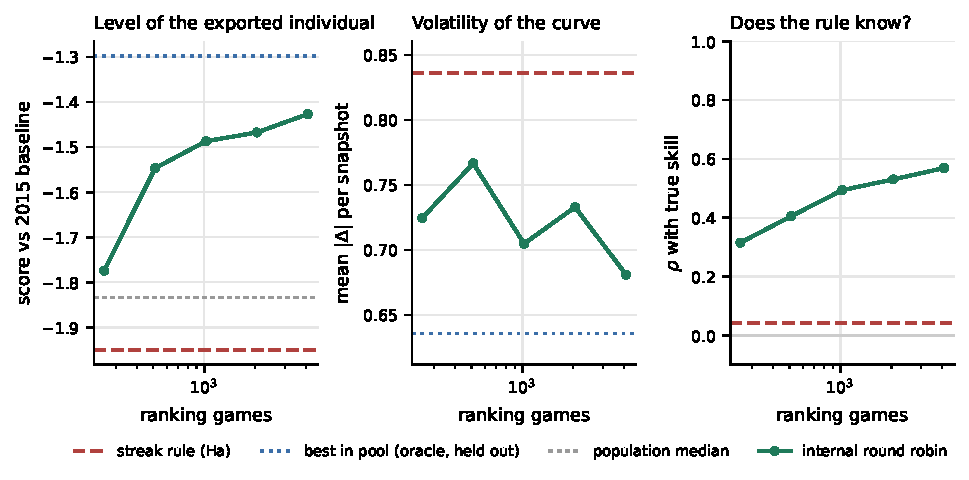
\includegraphics[width=0.9\linewidth]{figures/fig9_reexport.pdf}
\caption{Promotion rules as a function of the games spent ranking.}
\end{figure}

\begin{figure}[h]
\centering
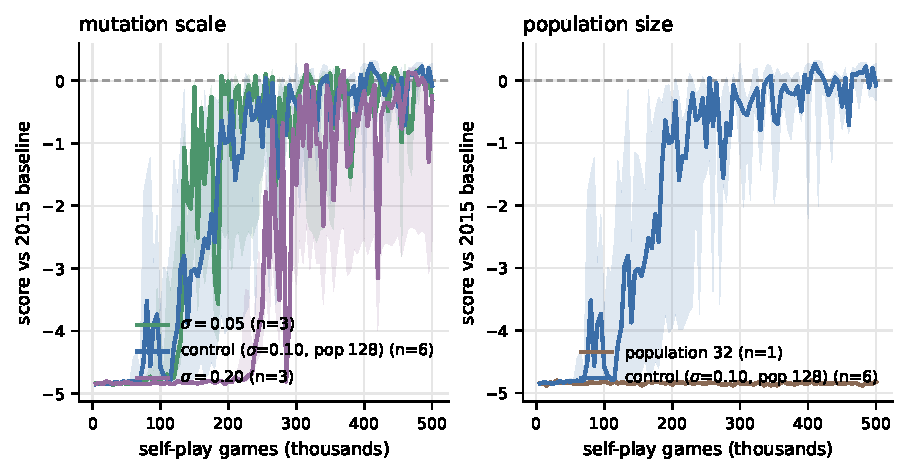
\includegraphics[width=0.9\linewidth]{figures/fig4_ablations.pdf}
\caption{Mutation scale and population size against the control.}
\end{figure}

\begin{figure}[h]
\centering
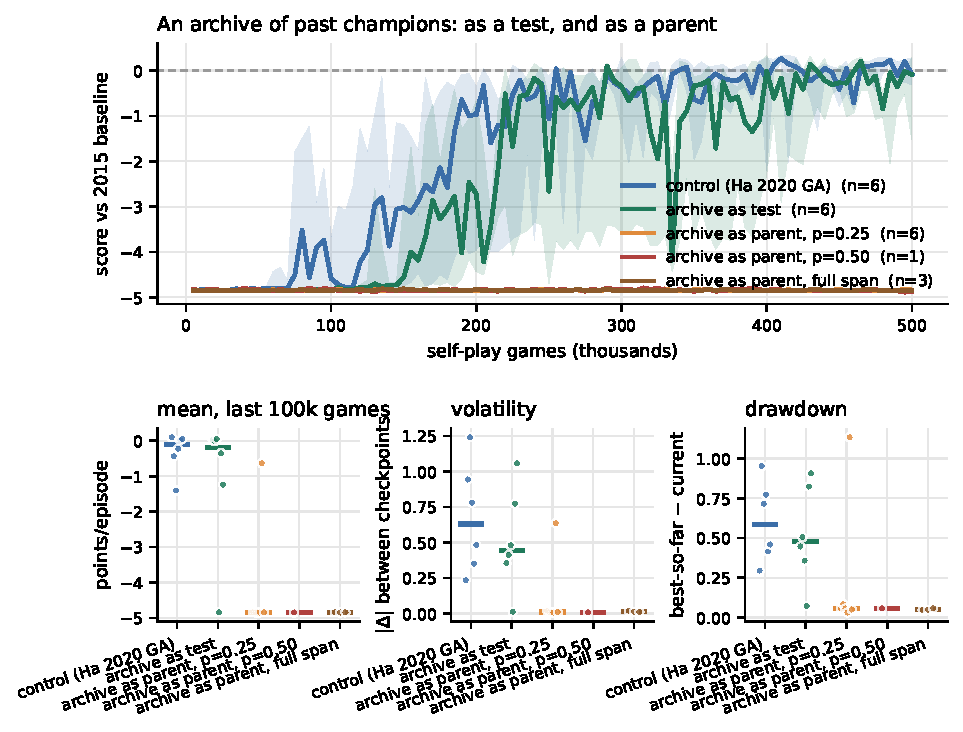
\includegraphics[width=0.9\linewidth]{figures/fig3_hall_of_fame.pdf}
\caption{The archive conditions against the control.}
\end{figure}

\end{document}
